% Options for packages loaded elsewhere
\PassOptionsToPackage{unicode}{hyperref}
\PassOptionsToPackage{hyphens}{url}
%
\documentclass[
]{book}
\usepackage{amsmath,amssymb}
\usepackage{lmodern}
\usepackage{iftex}
\ifPDFTeX
  \usepackage[T1]{fontenc}
  \usepackage[utf8]{inputenc}
  \usepackage{textcomp} % provide euro and other symbols
\else % if luatex or xetex
  \usepackage{unicode-math}
  \defaultfontfeatures{Scale=MatchLowercase}
  \defaultfontfeatures[\rmfamily]{Ligatures=TeX,Scale=1}
\fi
% Use upquote if available, for straight quotes in verbatim environments
\IfFileExists{upquote.sty}{\usepackage{upquote}}{}
\IfFileExists{microtype.sty}{% use microtype if available
  \usepackage[]{microtype}
  \UseMicrotypeSet[protrusion]{basicmath} % disable protrusion for tt fonts
}{}
\makeatletter
\@ifundefined{KOMAClassName}{% if non-KOMA class
  \IfFileExists{parskip.sty}{%
    \usepackage{parskip}
  }{% else
    \setlength{\parindent}{0pt}
    \setlength{\parskip}{6pt plus 2pt minus 1pt}}
}{% if KOMA class
  \KOMAoptions{parskip=half}}
\makeatother
\usepackage{xcolor}
\IfFileExists{xurl.sty}{\usepackage{xurl}}{} % add URL line breaks if available
\IfFileExists{bookmark.sty}{\usepackage{bookmark}}{\usepackage{hyperref}}
\hypersetup{
  pdftitle={Diplomado de Econometría Financiera},
  pdfauthor={Benjamin Oliva y Emiliano Pérez Caullieres},
  hidelinks,
  pdfcreator={LaTeX via pandoc}}
\urlstyle{same} % disable monospaced font for URLs
\usepackage{color}
\usepackage{fancyvrb}
\newcommand{\VerbBar}{|}
\newcommand{\VERB}{\Verb[commandchars=\\\{\}]}
\DefineVerbatimEnvironment{Highlighting}{Verbatim}{commandchars=\\\{\}}
% Add ',fontsize=\small' for more characters per line
\usepackage{framed}
\definecolor{shadecolor}{RGB}{248,248,248}
\newenvironment{Shaded}{\begin{snugshade}}{\end{snugshade}}
\newcommand{\AlertTok}[1]{\textcolor[rgb]{0.94,0.16,0.16}{#1}}
\newcommand{\AnnotationTok}[1]{\textcolor[rgb]{0.56,0.35,0.01}{\textbf{\textit{#1}}}}
\newcommand{\AttributeTok}[1]{\textcolor[rgb]{0.77,0.63,0.00}{#1}}
\newcommand{\BaseNTok}[1]{\textcolor[rgb]{0.00,0.00,0.81}{#1}}
\newcommand{\BuiltInTok}[1]{#1}
\newcommand{\CharTok}[1]{\textcolor[rgb]{0.31,0.60,0.02}{#1}}
\newcommand{\CommentTok}[1]{\textcolor[rgb]{0.56,0.35,0.01}{\textit{#1}}}
\newcommand{\CommentVarTok}[1]{\textcolor[rgb]{0.56,0.35,0.01}{\textbf{\textit{#1}}}}
\newcommand{\ConstantTok}[1]{\textcolor[rgb]{0.00,0.00,0.00}{#1}}
\newcommand{\ControlFlowTok}[1]{\textcolor[rgb]{0.13,0.29,0.53}{\textbf{#1}}}
\newcommand{\DataTypeTok}[1]{\textcolor[rgb]{0.13,0.29,0.53}{#1}}
\newcommand{\DecValTok}[1]{\textcolor[rgb]{0.00,0.00,0.81}{#1}}
\newcommand{\DocumentationTok}[1]{\textcolor[rgb]{0.56,0.35,0.01}{\textbf{\textit{#1}}}}
\newcommand{\ErrorTok}[1]{\textcolor[rgb]{0.64,0.00,0.00}{\textbf{#1}}}
\newcommand{\ExtensionTok}[1]{#1}
\newcommand{\FloatTok}[1]{\textcolor[rgb]{0.00,0.00,0.81}{#1}}
\newcommand{\FunctionTok}[1]{\textcolor[rgb]{0.00,0.00,0.00}{#1}}
\newcommand{\ImportTok}[1]{#1}
\newcommand{\InformationTok}[1]{\textcolor[rgb]{0.56,0.35,0.01}{\textbf{\textit{#1}}}}
\newcommand{\KeywordTok}[1]{\textcolor[rgb]{0.13,0.29,0.53}{\textbf{#1}}}
\newcommand{\NormalTok}[1]{#1}
\newcommand{\OperatorTok}[1]{\textcolor[rgb]{0.81,0.36,0.00}{\textbf{#1}}}
\newcommand{\OtherTok}[1]{\textcolor[rgb]{0.56,0.35,0.01}{#1}}
\newcommand{\PreprocessorTok}[1]{\textcolor[rgb]{0.56,0.35,0.01}{\textit{#1}}}
\newcommand{\RegionMarkerTok}[1]{#1}
\newcommand{\SpecialCharTok}[1]{\textcolor[rgb]{0.00,0.00,0.00}{#1}}
\newcommand{\SpecialStringTok}[1]{\textcolor[rgb]{0.31,0.60,0.02}{#1}}
\newcommand{\StringTok}[1]{\textcolor[rgb]{0.31,0.60,0.02}{#1}}
\newcommand{\VariableTok}[1]{\textcolor[rgb]{0.00,0.00,0.00}{#1}}
\newcommand{\VerbatimStringTok}[1]{\textcolor[rgb]{0.31,0.60,0.02}{#1}}
\newcommand{\WarningTok}[1]{\textcolor[rgb]{0.56,0.35,0.01}{\textbf{\textit{#1}}}}
\usepackage{longtable,booktabs,array}
\usepackage{calc} % for calculating minipage widths
% Correct order of tables after \paragraph or \subparagraph
\usepackage{etoolbox}
\makeatletter
\patchcmd\longtable{\par}{\if@noskipsec\mbox{}\fi\par}{}{}
\makeatother
% Allow footnotes in longtable head/foot
\IfFileExists{footnotehyper.sty}{\usepackage{footnotehyper}}{\usepackage{footnote}}
\makesavenoteenv{longtable}
\usepackage{graphicx}
\makeatletter
\def\maxwidth{\ifdim\Gin@nat@width>\linewidth\linewidth\else\Gin@nat@width\fi}
\def\maxheight{\ifdim\Gin@nat@height>\textheight\textheight\else\Gin@nat@height\fi}
\makeatother
% Scale images if necessary, so that they will not overflow the page
% margins by default, and it is still possible to overwrite the defaults
% using explicit options in \includegraphics[width, height, ...]{}
\setkeys{Gin}{width=\maxwidth,height=\maxheight,keepaspectratio}
% Set default figure placement to htbp
\makeatletter
\def\fps@figure{htbp}
\makeatother
\setlength{\emergencystretch}{3em} % prevent overfull lines
\providecommand{\tightlist}{%
  \setlength{\itemsep}{0pt}\setlength{\parskip}{0pt}}
\setcounter{secnumdepth}{5}
\usepackage{booktabs}
\ifLuaTeX
  \usepackage{selnolig}  % disable illegal ligatures
\fi
\usepackage[]{natbib}
\bibliographystyle{apalike}

\title{Diplomado de Econometría Financiera}
\author{Benjamin Oliva y Emiliano Pérez Caullieres}
\date{2022-08-19}

\begin{document}
\maketitle

{
\setcounter{tocdepth}{1}
\tableofcontents
}
\hypertarget{muxednimos-cuadrados-ordinarios}{%
\chapter{Mínimos Cuadrados Ordinarios}\label{muxednimos-cuadrados-ordinarios}}

\hypertarget{el-problema}{%
\section{El problema}\label{el-problema}}

Recrodando que el método de MCO resulta en encontrar la combinación de valores de los estimadores de los parámetros \(\hat{\boldsymbol{\beta}}\) que permita minimizar la suma de los residuales (estimadores de los términos de erro \(\boldsymbol{\varepsilon}\)) al cuadrado dada por:

\[
    \sum^{N}_{i=1}{e^2_i} = \sum^{N}_{i = 1}{(y_i - \mathbf{X}'_i \hat{\boldsymbol{\beta}})^2}
\]

Donde \(\hat{\boldsymbol{\beta}}\) denota el vector de estimadores \(\hat{\beta}_1, \ldots, \hat{\beta}_K\) y dado que \((e_1, e_2, \ldots, e_n)'(e_1, e_2, \ldots, e_n) = {\mathbf{e'e}}\), el problema del método de MCO consiste en resolver el problema de óptimización:

\begin{eqnarray*}
Minimizar_{\hat{\boldsymbol \beta}} S(\hat{\boldsymbol \beta})  =  Minimizar_{\hat{\boldsymbol \beta}} \mathbf{e'e} \\
    =  Minimizar_{\hat{\boldsymbol \beta}} (\mathbf{Y}-\mathbf{X}\hat{\boldsymbol \beta})'(\mathbf{Y}-\mathbf{X}\hat{\boldsymbol \beta})
\end{eqnarray*}

Expandiendo la expresión \(\mathbf{e'e}\) obtenemos:
\[
    \mathbf{e'e} = \mathbf{Y'Y} - 2 \mathbf{Y'X} \hat{\boldsymbol \beta} + \hat{\boldsymbol \beta}' \mathbf{X'X}\hat{\boldsymbol \beta}
\]

De esta forma obtenemos que las condiciones necesarias de un mínimo son:

\[
    \frac{\partial S(\hat{\boldsymbol \beta})}{\partial \hat{\boldsymbol \beta}} = -2{\mathbf{X'Y}} + 2{\mathbf{X'X}} \hat{\boldsymbol{\beta}} = \mathbf{0}
\]
Y se pueden despejar las \textit{ecuaciones normales} dadas por:

Debido a que el objetivo es encontrar la matriz \(\hat{\boldsymbol\beta}\) despejamos:

\[\hat{\boldsymbol \beta} = (\mathbf{X'X})^{-1}\mathbf{X'Y}
\]
\[
    \mathbf{X'X}\hat{\boldsymbol \beta} = \mathbf{X'Y}
\]

\hypertarget{estimaciuxf3n}{%
\section{Estimación}\label{estimaciuxf3n}}

Para la estimación utilizaremos el paquete ``BatchGetSymbols''. Este paquete nos permitirá descargar información acerca de la bolsa de valores internacional.

\hypertarget{dependencias}{%
\subsection{Dependencias}\label{dependencias}}

\begin{Shaded}
\begin{Highlighting}[]
\CommentTok{\#install.packages("pacman")}
\CommentTok{\#pacman nos permite cargar varias librerias en una sola línea}
\FunctionTok{library}\NormalTok{(pacman)}
\NormalTok{pacman}\SpecialCharTok{::}\FunctionTok{p\_load}\NormalTok{(tidyverse,BatchGetSymbols,ggplot2, lubridate)}
\end{Highlighting}
\end{Shaded}

\hypertarget{descarga-de-los-valores}{%
\subsection{Descarga de los valores}\label{descarga-de-los-valores}}

\begin{Shaded}
\begin{Highlighting}[]
\CommentTok{\#Primero determinamos el lapso de tiempo}
\NormalTok{pd}\OtherTok{\textless{}{-}}\FunctionTok{Sys.Date}\NormalTok{()}\SpecialCharTok{{-}}\DecValTok{365} \CommentTok{\#primer fecha}
\NormalTok{pd}
\CommentTok{\#\textgreater{} [1] "2021{-}08{-}19"}
\NormalTok{ld}\OtherTok{\textless{}{-}}\FunctionTok{Sys.Date}\NormalTok{() }\CommentTok{\#última fecha}
\NormalTok{ld}
\CommentTok{\#\textgreater{} [1] "2022{-}08{-}19"}
\CommentTok{\#Intervalos de tiempo}
\NormalTok{int}\OtherTok{\textless{}{-}}\StringTok{"monthly"}
\CommentTok{\#Datos a elegir}
\NormalTok{dt}\OtherTok{\textless{}{-}}\FunctionTok{c}\NormalTok{(}\StringTok{"AMZN"}\NormalTok{)}
\CommentTok{\#Descargando los valores}
\NormalTok{?}\FunctionTok{BatchGetSymbols}\NormalTok{()}
\NormalTok{data}\OtherTok{\textless{}{-}} \FunctionTok{BatchGetSymbols}\NormalTok{(}\AttributeTok{tickers =}\NormalTok{ dt,}
                       \AttributeTok{first.date =}\NormalTok{ pd,}
                       \AttributeTok{last.date =}\NormalTok{ ld,}
                       \AttributeTok{freq.data =}\NormalTok{ int,}
                       \AttributeTok{do.cache =} \ConstantTok{FALSE}\NormalTok{,}
                       \AttributeTok{thresh.bad.data =} \DecValTok{0}\NormalTok{)}
\CommentTok{\#Generando data frame con los valores}
\NormalTok{data\_precio}\OtherTok{\textless{}{-}}\NormalTok{data}\SpecialCharTok{$}\NormalTok{df.tickers}
\end{Highlighting}
\end{Shaded}

\hypertarget{gruxe1ficas}{%
\subsection{Gráficas}\label{gruxe1ficas}}

\begin{Shaded}
\begin{Highlighting}[]
\NormalTok{sp\_precio}\OtherTok{\textless{}{-}}\FunctionTok{ggplot}\NormalTok{(data\_precio, }\FunctionTok{aes}\NormalTok{(}\AttributeTok{x=}\NormalTok{ref.date, }\AttributeTok{y=}\NormalTok{price.open))}\SpecialCharTok{+}\FunctionTok{geom\_point}\NormalTok{(}\AttributeTok{size =}\DecValTok{2}\NormalTok{, }\AttributeTok{colour =} \StringTok{"black"}\NormalTok{)}\SpecialCharTok{+}\FunctionTok{labs}\NormalTok{(}\AttributeTok{x=}\StringTok{"Fecha"}\NormalTok{, }\AttributeTok{y=}\StringTok{"Precio de apertura (USD)"}\NormalTok{, }\AttributeTok{title=}\StringTok{"Precio de apertura de AMZN en el ultimo año"}\NormalTok{)}\SpecialCharTok{+} \FunctionTok{theme\_light}\NormalTok{()}
\NormalTok{sp\_precio}
\end{Highlighting}
\end{Shaded}

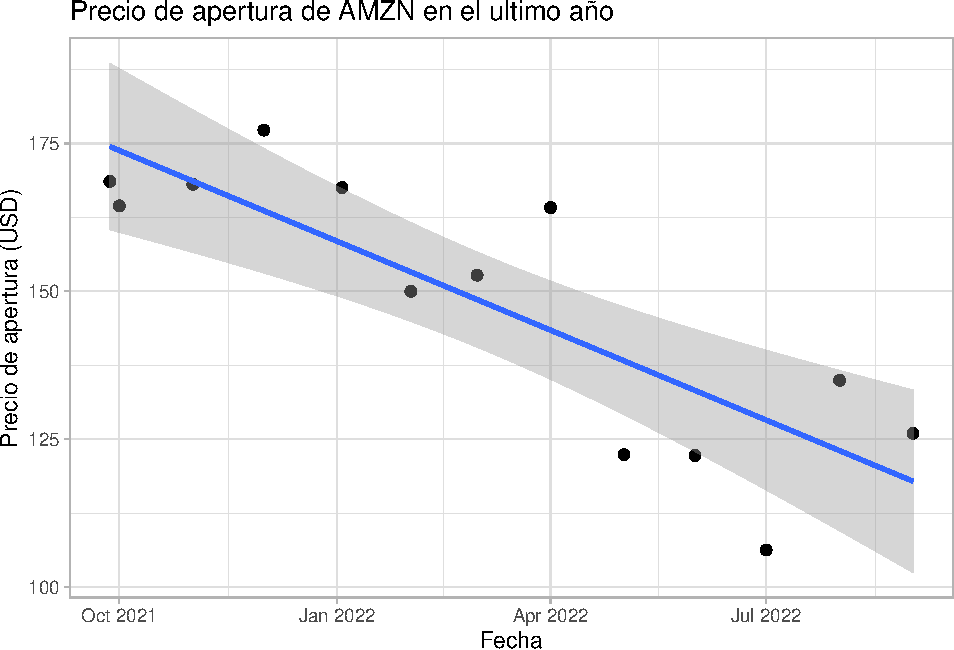
\includegraphics{index_files/figure-latex/unnamed-chunk-3-1.pdf}

\begin{Shaded}
\begin{Highlighting}[]

\NormalTok{sp\_volumen}\OtherTok{\textless{}{-}}\FunctionTok{ggplot}\NormalTok{(data\_precio, }\FunctionTok{aes}\NormalTok{(}\AttributeTok{x=}\NormalTok{ref.date, }\AttributeTok{y=}\NormalTok{volume))}\SpecialCharTok{+}\FunctionTok{geom\_point}\NormalTok{(}\AttributeTok{size =}\DecValTok{2}\NormalTok{, }\AttributeTok{colour =} \StringTok{"black"}\NormalTok{)}\SpecialCharTok{+}\FunctionTok{labs}\NormalTok{(}\AttributeTok{x=}\StringTok{"Fecha"}\NormalTok{, }\AttributeTok{y=}\StringTok{"Volumen"}\NormalTok{, }\AttributeTok{title=}\StringTok{"Volumenes de AMZN en el ultimo año"}\NormalTok{)}\SpecialCharTok{+} \FunctionTok{theme\_light}\NormalTok{()}
\NormalTok{sp\_volumen}
\end{Highlighting}
\end{Shaded}

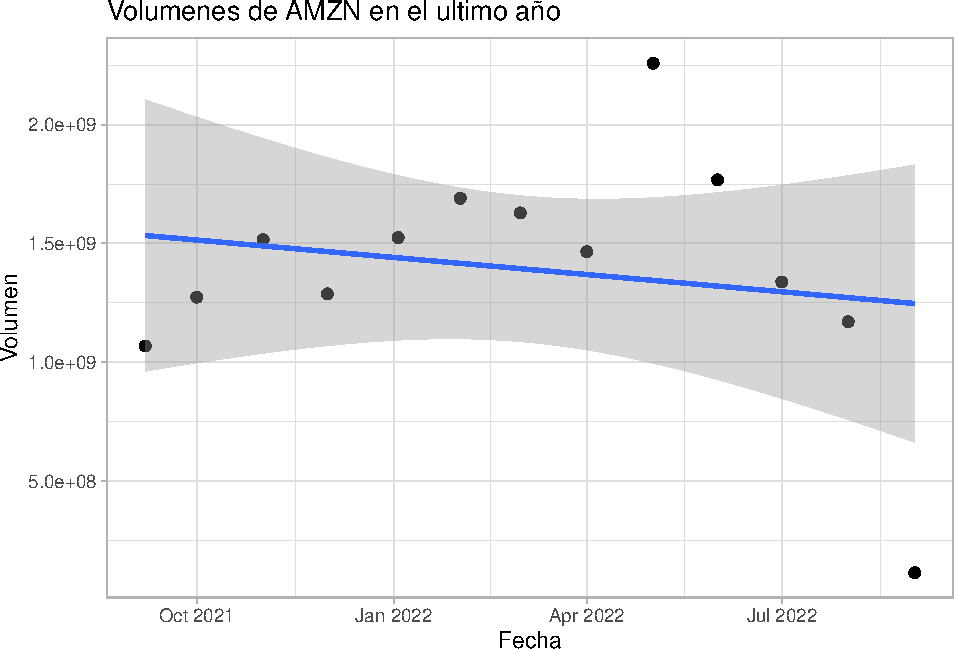
\includegraphics{index_files/figure-latex/unnamed-chunk-3-2.pdf}

\hypertarget{regresiuxf3n-lineal-que-optiene-los-coeficientes-hatboldsymbol-beta}{%
\subsection{\texorpdfstring{Regresión lineal que optiene los coeficientes \(\hat{\boldsymbol \beta}\)}{Regresión lineal que optiene los coeficientes \textbackslash hat\{\textbackslash boldsymbol \textbackslash beta\}}}\label{regresiuxf3n-lineal-que-optiene-los-coeficientes-hatboldsymbol-beta}}

\begin{Shaded}
\begin{Highlighting}[]
\CommentTok{\#datos estadísticos}
\FunctionTok{summary}\NormalTok{(data\_precio[}\FunctionTok{c}\NormalTok{(}\StringTok{"price.open"}\NormalTok{,}\StringTok{"volume"}\NormalTok{)])}
\CommentTok{\#\textgreater{}    price.open        volume         }
\CommentTok{\#\textgreater{}  Min.   :106.3   Min.   :5.338e+08  }
\CommentTok{\#\textgreater{}  1st Qu.:135.0   1st Qu.:1.273e+09  }
\CommentTok{\#\textgreater{}  Median :159.7   Median :1.465e+09  }
\CommentTok{\#\textgreater{}  Mean   :151.1   Mean   :1.407e+09  }
\CommentTok{\#\textgreater{}  3rd Qu.:167.6   3rd Qu.:1.628e+09  }
\CommentTok{\#\textgreater{}  Max.   :177.2   Max.   :2.258e+09}
\CommentTok{\#análisis de regresión lineal lm() y=precio,x=fecha}
\NormalTok{reg\_tiempo\_precio}\OtherTok{\textless{}{-}}\FunctionTok{lm}\NormalTok{(price.open}\SpecialCharTok{\textasciitilde{}}\NormalTok{ref.date, }\AttributeTok{data=}\NormalTok{data\_precio)}
\FunctionTok{summary}\NormalTok{(reg\_tiempo\_precio)}
\CommentTok{\#\textgreater{} }
\CommentTok{\#\textgreater{} Call:}
\CommentTok{\#\textgreater{} lm(formula = price.open \textasciitilde{} ref.date, data = data\_precio)}
\CommentTok{\#\textgreater{} }
\CommentTok{\#\textgreater{} Residuals:}
\CommentTok{\#\textgreater{}      Min       1Q   Median       3Q      Max }
\CommentTok{\#\textgreater{} {-}21.4042 {-}10.1319  {-}0.2814  11.8496  22.2175 }
\CommentTok{\#\textgreater{} }
\CommentTok{\#\textgreater{} Coefficients:}
\CommentTok{\#\textgreater{}               Estimate Std. Error t value Pr(\textgreater{}|t|)    }
\CommentTok{\#\textgreater{} (Intercept) 3127.64731  671.24128   4.659 0.000694 ***}
\CommentTok{\#\textgreater{} ref.date      {-}0.15646    0.03528  {-}4.434 0.001004 ** }
\CommentTok{\#\textgreater{} {-}{-}{-}}
\CommentTok{\#\textgreater{} Signif. codes:  }
\CommentTok{\#\textgreater{} 0 \textquotesingle{}***\textquotesingle{} 0.001 \textquotesingle{}**\textquotesingle{} 0.01 \textquotesingle{}*\textquotesingle{} 0.05 \textquotesingle{}.\textquotesingle{} 0.1 \textquotesingle{} \textquotesingle{} 1}
\CommentTok{\#\textgreater{} }
\CommentTok{\#\textgreater{} Residual standard error: 14.17 on 11 degrees of freedom}
\CommentTok{\#\textgreater{} Multiple R{-}squared:  0.6413, Adjusted R{-}squared:  0.6087 }
\CommentTok{\#\textgreater{} F{-}statistic: 19.66 on 1 and 11 DF,  p{-}value: 0.001004}

\CommentTok{\#análisis de regresión lineal lm() y=volumen,x=fecha}
\NormalTok{reg\_tiempo\_volumen}\OtherTok{\textless{}{-}}\FunctionTok{lm}\NormalTok{(volume}\SpecialCharTok{\textasciitilde{}}\NormalTok{ref.date, }\AttributeTok{data=}\NormalTok{data\_precio)}
\FunctionTok{summary}\NormalTok{(reg\_tiempo\_volumen)}
\CommentTok{\#\textgreater{} }
\CommentTok{\#\textgreater{} Call:}
\CommentTok{\#\textgreater{} lm(formula = volume \textasciitilde{} ref.date, data = data\_precio)}
\CommentTok{\#\textgreater{} }
\CommentTok{\#\textgreater{} Residuals:}
\CommentTok{\#\textgreater{}        Min         1Q     Median         3Q        Max }
\CommentTok{\#\textgreater{} {-}853671262  {-}49527288   15223912  212399437  751223038 }
\CommentTok{\#\textgreater{} }
\CommentTok{\#\textgreater{} Coefficients:}
\CommentTok{\#\textgreater{}               Estimate Std. Error t value Pr(\textgreater{}|t|)}
\CommentTok{\#\textgreater{} (Intercept) {-}1.988e+10  2.050e+10  {-}0.970    0.353}
\CommentTok{\#\textgreater{} ref.date     1.119e+06  1.077e+06   1.039    0.321}
\CommentTok{\#\textgreater{} }
\CommentTok{\#\textgreater{} Residual standard error: 432700000 on 11 degrees of freedom}
\CommentTok{\#\textgreater{} Multiple R{-}squared:  0.0893, Adjusted R{-}squared:  0.006508 }
\CommentTok{\#\textgreater{} F{-}statistic: 1.079 on 1 and 11 DF,  p{-}value: 0.3213}
\end{Highlighting}
\end{Shaded}

\hypertarget{hello-bookdown}{%
\chapter{Hello bookdown}\label{hello-bookdown}}

All chapters start with a first-level heading followed by your chapter title, like the line above. There should be only one first-level heading (\texttt{\#}) per .Rmd file.

\hypertarget{a-section}{%
\section{A section}\label{a-section}}

All chapter sections start with a second-level (\texttt{\#\#}) or higher heading followed by your section title, like the sections above and below here. You can have as many as you want within a chapter.

\hypertarget{an-unnumbered-section}{%
\subsection*{An unnumbered section}\label{an-unnumbered-section}}
\addcontentsline{toc}{subsection}{An unnumbered section}

Chapters and sections are numbered by default. To un-number a heading, add a \texttt{\{.unnumbered\}} or the shorter \texttt{\{-\}} at the end of the heading, like in this section.

  \bibliography{book.bib,packages.bib}

\end{document}
